\documentclass[UTF8]{ctexart}
\CTEXsetup[format={\Large\bfseries}]{section}
\setCJKmainfont{KaiTi}
\setmainfont{Times New Roman}
\usepackage{geometry}
\geometry{a4paper, left=3.4cm, right=3.4cm, top=2.4cm, bottom=2.4cm}
%\geometry{a4paper, scale=0.75}
%\usepackage{setspace}
%\onehalfspacing
\addtolength{\parskip}{-0.1em}
\usepackage{amsmath}
\usepackage{ulem}
\usepackage{graphicx}
\usepackage{float}
\usepackage{subfigure}
\usepackage{fancyhdr}
\pagestyle{plain}
\usepackage{caption}
\renewcommand{\figurename}{Figure}
\usepackage[colorlinks,linkcolor=blue,anchorcolor=blue, citecolor=blue, bookmarks, bookmarksopen, pdfstartview=FitH]{hyperref} 
\usepackage{listings}
\usepackage{xcolor}
\usepackage{fontspec}
\usepackage{algorithm}
\usepackage{algorithmicx}
\usepackage{algpseudocode}
\definecolor{mygreen}{rgb}{0,0.6,0}  
\definecolor{mygray}{rgb}{0.5,0.5,0.5}  
\definecolor{mymauve}{rgb}{0.58,0,0.82}  

\lstset{ %  
	basicstyle={\fontspec{Consolas} \footnotesize},
	backgroundcolor=\color{white},   % choose the background color; you must add \usepackage{color} or \usepackage{xcolor}  
%	basicstyle=\footnotesize,        % the size of the fonts that are used for the code  
	breakatwhitespace=false,         % sets if automatic breaks should only happen at whitespace  
	breaklines=true,                 % sets automatic line breaking  
	captionpos=bl,                    % sets the caption-position to bottom  
	commentstyle=\color{mygreen},    % comment style  
	deletekeywords={...},            % if you want to delete keywords from the given language  
	escapeinside={\%*}{*)},          % if you want to add LaTeX within your code  
	extendedchars=true,              % lets you use non-ASCII characters; for 8-bits encodings only, does not work with UTF-8  
	frame=single,                    % adds a frame around the code  
%	keepspaces=true,                 % keeps spaces in text, useful for keeping indentation of code (possibly needs columns=flexible)  
	keywordstyle=\color{blue},       % keyword style  
	%language=Python,                 % the language of the code  
	morekeywords={*,...},            % if you want to add more keywords to the set  
	numbers=left,                    % where to put the line-numbers; possible values are (none, left, right)  
	numbersep=5pt,                   % how far the line-numbers are from the code  
	numberstyle=\tiny\color{mygray}, % the style that is used for the line-numbers  
	rulecolor=\color{black},         % if not set, the frame-color may be changed on line-breaks within not-black text (e.g. comments (green here))  
	showspaces=false,                % show spaces everywhere adding particular underscores; it overrides 'showstringspaces'  
	showstringspaces=false,          % underline spaces within strings only  
	showtabs=false,                  % show tabs within strings adding particular underscores  
	stepnumber=1,                    % the step between two line-numbers. If it's 1, each line will be numbered  
	stringstyle=\color{orange},     % string literal style  
	tabsize=2,                       % sets default tabsize to 2 spaces  
	%title=myPython.py                   % show the filename of files included with \lstinputlisting; also try caption instead of title  
}  

\makeatletter
\newenvironment{breakablealgorithm}
{% \begin{breakablealgorithm}
	\begin{center}
		\refstepcounter{algorithm}% New algorithm
		\hrule height.8pt depth0pt \kern2pt% \@fs@pre for \@fs@ruled
		\renewcommand{\caption}[2][\relax]{% Make a new \caption
			{\raggedright\textbf{\ALG@name~\thealgorithm} ##2\par}%
			\ifx\relax##1\relax % #1 is \relax
			\addcontentsline{loa}{algorithm}{\protect\numberline{\thealgorithm}##2}%
			\else % #1 is not \relax
			\addcontentsline{loa}{algorithm}{\protect\numberline{\thealgorithm}##1}%
			\fi
			\kern2pt\hrule\kern2pt
		}
	}{% \end{breakablealgorithm}
		\kern2pt\hrule\relax% \@fs@post for \@fs@ruled
	\end{center}
}
\makeatother

\title{Image Compression\footnote{https://github.com/sdc17/NaiveIC}}
\author{石大川\quad <sdc17@mails.tsinghua.edu.cn>}
\date{\today}
\begin{document}
	\maketitle
	\tableofcontents
%	\tableofcontents \newpage
	\section{1D-DCT \& 2D-DCT}
	
	\subsection{Principle}
	
	\paragraph{1D-DCT} 公式
	\begin{equation*}
	F(u) = c(u) \sum_{i=0}^{N-1}f(i)cos[\frac{(2i+1)\pi }{N}u] 
	\end{equation*}
	
	其中
	\begin{equation*}
	c(u) = \begin{cases}
	\sqrt{\frac{1}{N}}, \quad u=0 \\
	\sqrt{\frac{2}{N}}, \quad u \neq 0
	\end{cases}
	\end{equation*} 
	
	\paragraph{2D-DCT} 公式
	\begin{equation*}
	F(u, v) = c(u)c(v) \sum_{i=0}^{N-1}\sum_{j=0}^{N-1}f(i, j)cos[\frac{(2i+1)\pi }{2N}u]cos[\frac{(2j+1)\pi}{2N}v] 
	\end{equation*}
	
	其中
	\begin{equation*}
	c(u) = \begin{cases}
	\sqrt{\frac{1}{N}}, \quad u=0 \\
	\sqrt{\frac{2}{N}}, \quad u \neq 0
	\end{cases}
	\end{equation*} 
	\begin{equation*}
	c(v) = \begin{cases}
	\sqrt{\frac{1}{N}}, \quad v=0 \\
	\sqrt{\frac{2}{N}}, \quad v \neq 0
	\end{cases}
	\end{equation*} 
	
	实际做的时候写成矩阵形式
	\begin{equation*}
	G=\begin{bmatrix} \sqrt{\frac{1}{N}}[1&1&...&1]\\
	\sqrt{\frac{2}{N}}[[cos(\frac{\pi}{2N})]&[cos(\frac{3\pi}{2N})]&...&[cos(\frac{(2N-1)\pi}{2N})]] \\
	...&...&...&...\\
	\sqrt{\frac{2}{N}}[[cos(\frac{(N-1)\pi}{2N})]&[cos(\frac{(N-1)3\pi}{2N})]&...&[cos(\frac{(N-1)(2N-1)\pi}{2N})]]
	\end{bmatrix}
	\end{equation*}
	
	做1D-DCT时
	\begin{equation*}
	\textbf{F}=\textbf{G}\textbf{f}
	\end{equation*}
	
	2D-DCT时
	\begin{equation*}
	\textbf{F}=\textbf{G}\textbf{f}\textbf{G}^T
	\end{equation*}
	
	2D-DCT实际上等价于做两次1D-DCT
	
	\begin{equation*}
	\textbf{F} = \textbf{G}_{col}[\textbf{G}_{row}[\textbf{f}]^T]^T
	\end{equation*}
	
	\subsection{Results}
	
	\subsubsection{Comparison between two trials} 
	
	首先是两个trials对比见\hyperref[Fig.part1-1-1]{Figure 1},为了便于观察我对DCT的结果取了log,下同。
	
	\begin{figure}[htbp]
		\centering
		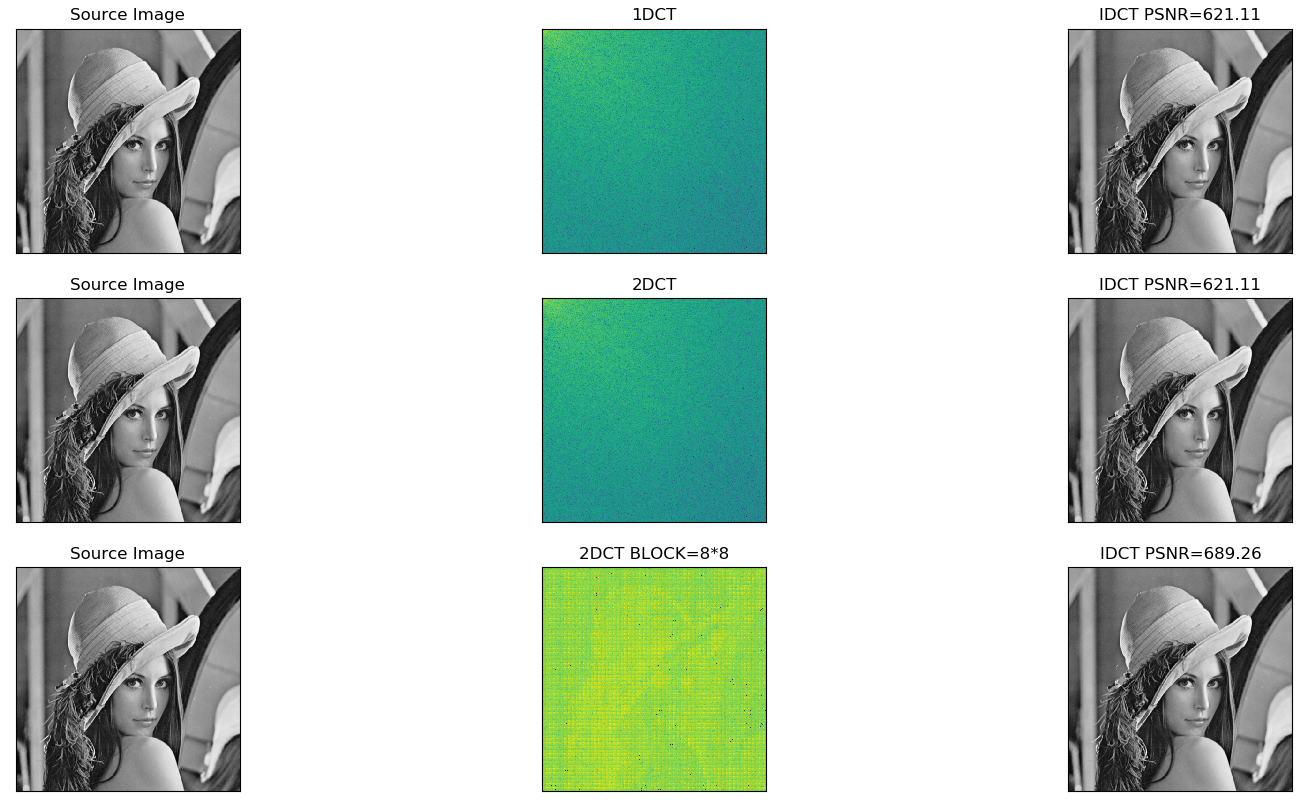
\includegraphics[width=1.0\textwidth]{../part1-1-1.png}
		\caption{1D-DCT and 2D-DCT}
		\label{Fig.part1-1-1}
	\end{figure}
	
	第一行和第二行分别是在全图上做1DCT和2DCT,PSNR值相等,可见在相同大小的图上做2次1DCT和1次2DCT是等价的,第三行是BLOCK SIZE为$8\times 8$的2DCT,可见BLOCK SIZE的大小这个变量是会影响PSNR的。
	
	当保留部分系数,如$\frac{1}{4}$时,1DCT先在行方向上保留$\frac{1}{2}$,再到列方向上保留$\frac{1}{2}$见\hyperref[Fig.part1-1-2]{Figure 2}
	\begin{figure}[htbp]
		\centering
		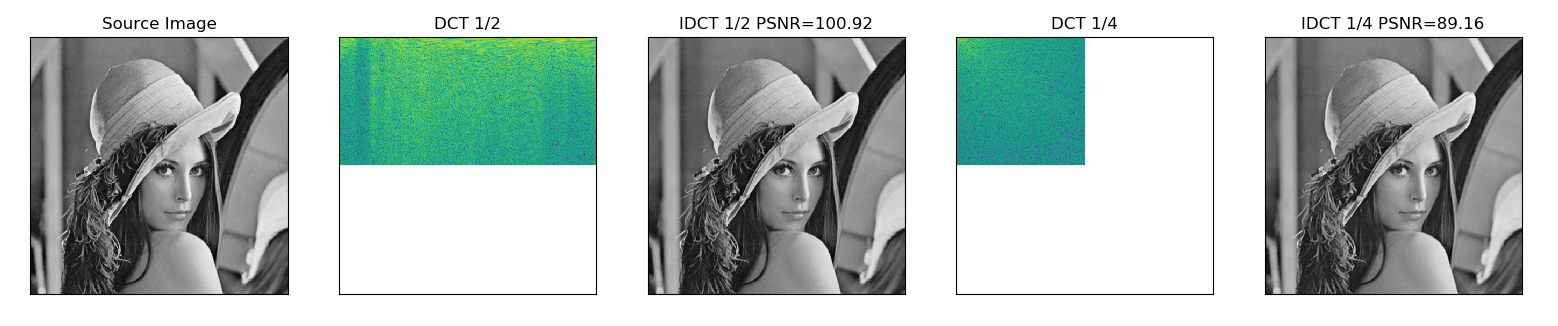
\includegraphics[width=1.0\textwidth]{../part1-1-2.png}
		\caption{1D-DCT(1/4)}
		\label{Fig.part1-1-2}
	\end{figure}

	和2DCT直接保留$\frac{1}{4}$的对比见\hyperref[Fig.part1-1-3]{Figure 3}
	\begin{figure}[htbp]
		\centering
		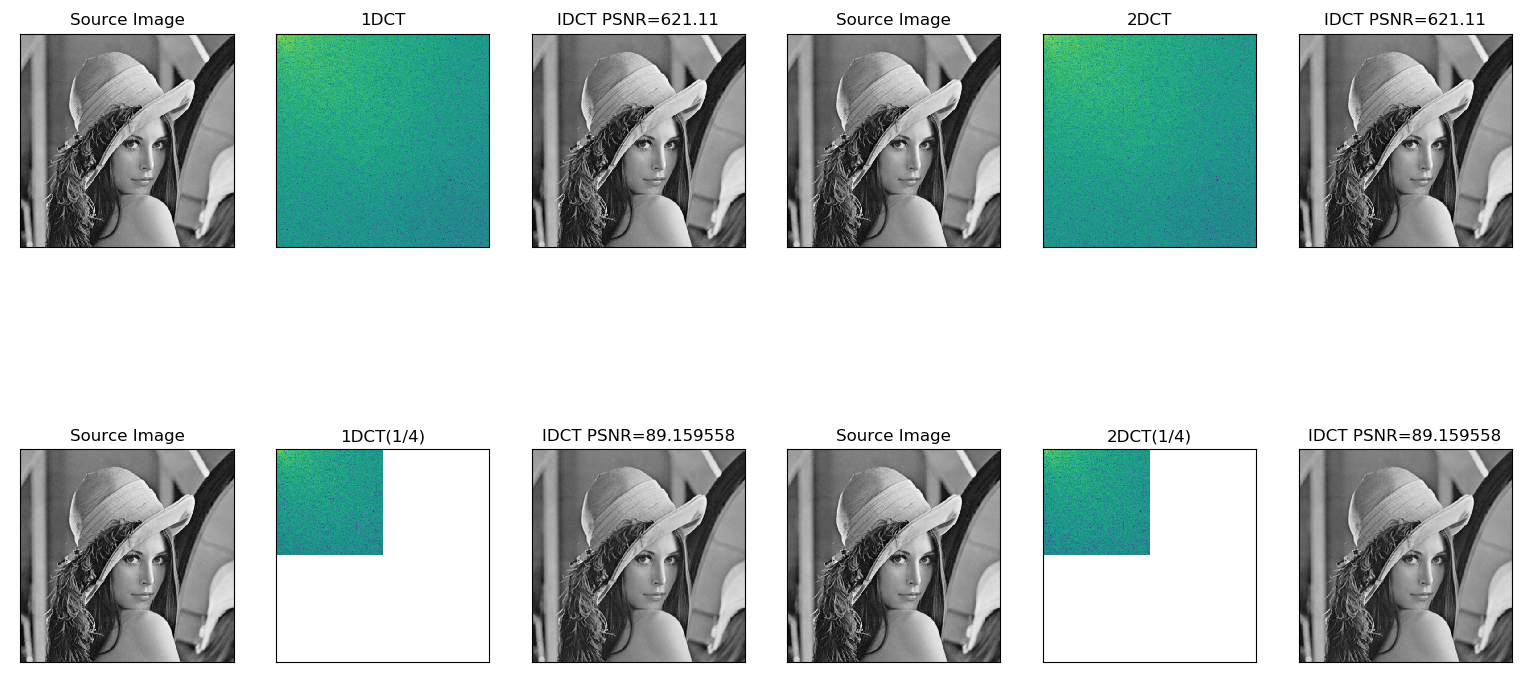
\includegraphics[width=1.0\textwidth]{../part1-1-3.png}
		\caption{1D-DCT(1/4) and 2D-DCT(1/4)}
		\label{Fig.part1-1-3}
	\end{figure}
	
	二者最终的PSNR在8位有效数字的精度下是相等的,可以认为1D-DCT和2D-DCT在8位有效数字的精度下,保留部分系数的结果也是等价的。
	
	\subsubsection{Different Coefficients}
	
	这里用BLOCK SIZE为$8\times 8$的2DCT来进行实验,见\hyperref[Fig.part1-2]{Figure 4}
	
	\begin{figure}[htbp]
		\centering
		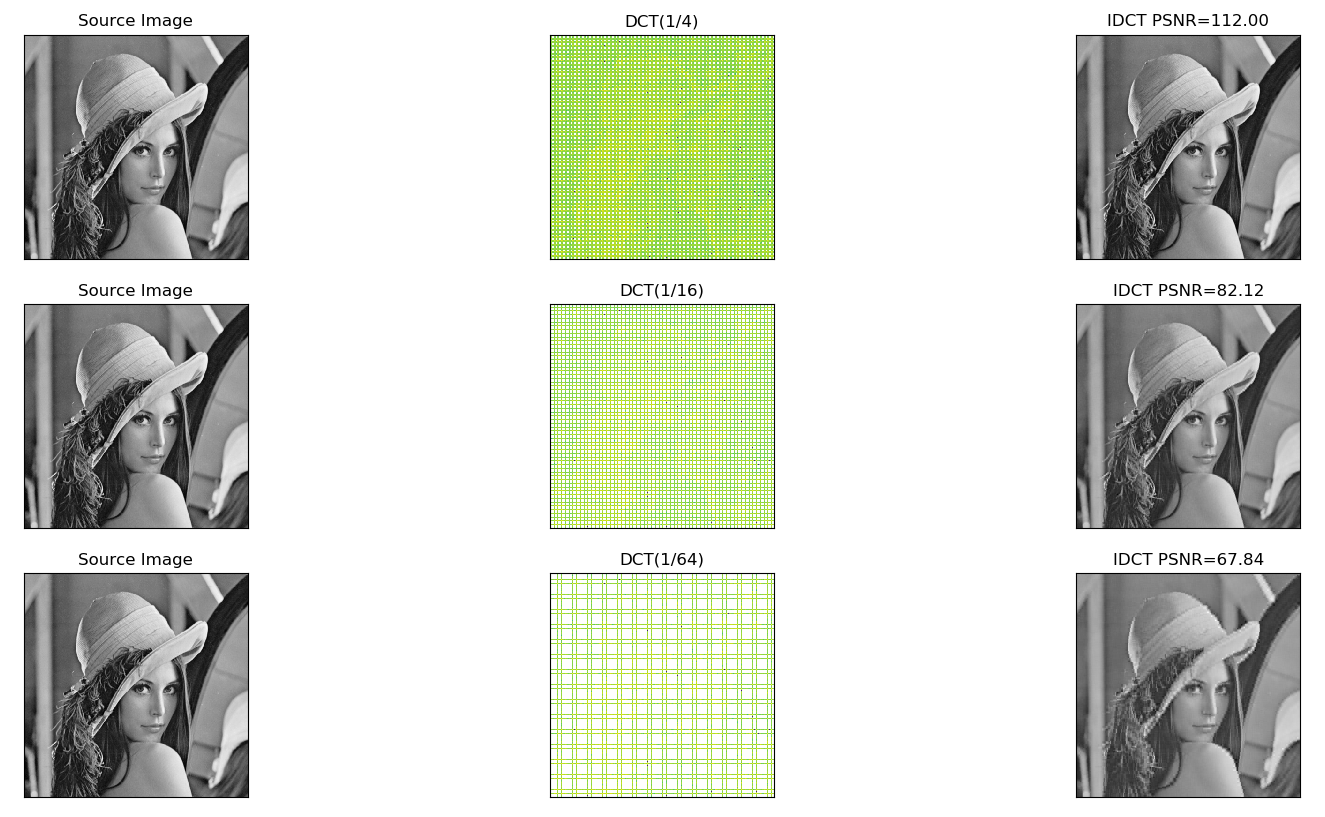
\includegraphics[width=1.0\textwidth]{../part1-2.png}
		\caption{Different Coefficients}
		\label{Fig.part1-2}
	\end{figure}

	可见随着保留下来的系数的减少,PSNR下降了且DCT的结果在观感上变得更稀疏了,IDCT的结果在观感上变得更加模糊了,这是符合逻辑的。
	
	\subsubsection{Different Block Size}
	
	这里用保留全部系数的2DCT来进行实验,见\hyperref[Fig.part1-3-1]{Figure 5}
	
	有一个实现上的细节是当原图边长不能整除Block边长时可以将原图padding到刚好整除,做完DCT和IDCT后再裁剪回原来的大小即可。
	
	\begin{figure}[htbp]
		\centering
		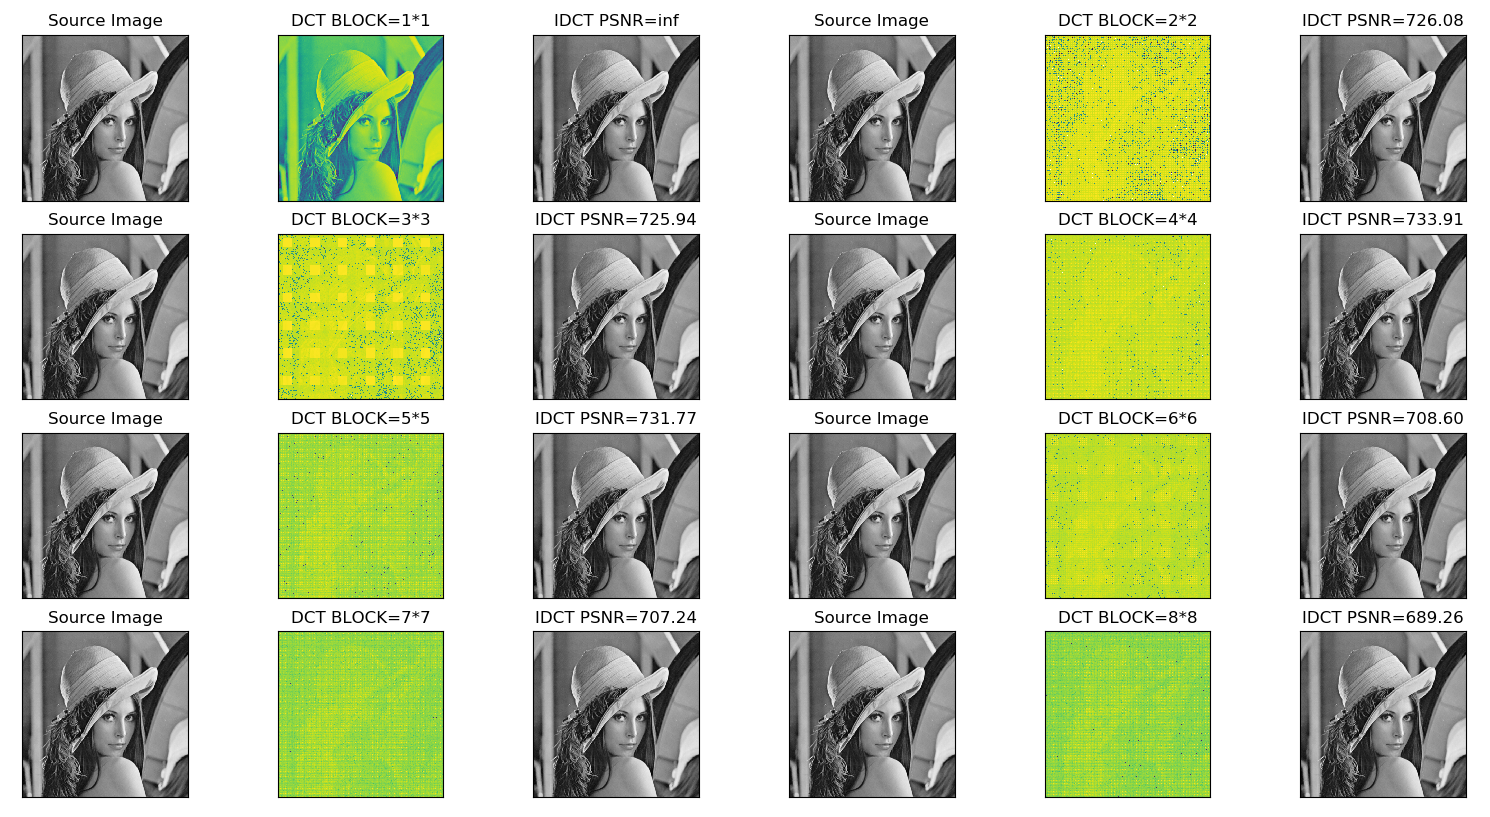
\includegraphics[width=1.0\textwidth]{../part1-3-1.png}
		\caption{Different Coefficients}
		\label{Fig.part1-3-1}
	\end{figure}

	相应的折线图见\hyperref[Fig.part1-3-2]{Figure 6}
	
	\begin{figure}[htbp]
		\centering
		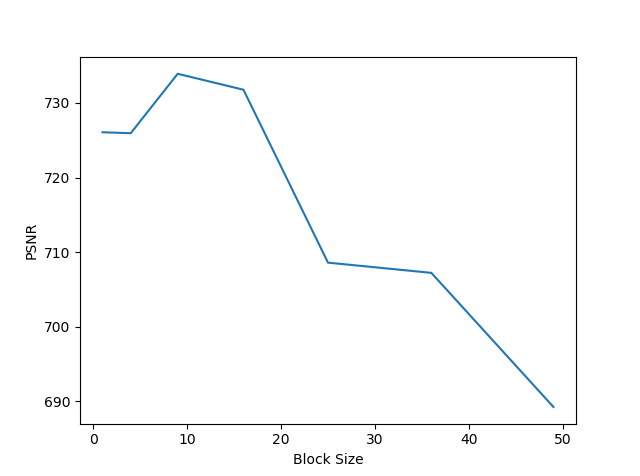
\includegraphics[width=1.0\textwidth]{../part1-3-2.png}
		\caption{Different Coefficients}
		\label{Fig.part1-3-2}
	\end{figure}
	
	可见总体上随着Block Size的增大,PSNR是会下降的。特别地,当Block Size为$1\times 1$时做的是pixelwise的DCT,此时MSE为0,PSNR为inf,当Block Size为原图尺寸时,也即\hyperref[Fig.part1-1-1]{Figure 1}中对全图做的2DCT,PSNR取得最小(或接近最小),这些结果是符合逻辑的。
	
	\section{Quantization}
	
	\subsection{Principle}
	公式很简洁,Quantization时
	\begin{equation*}
	C_q(u,v)=Round[\frac{C(u, v)}{Q(u, v)}]
	\end{equation*}
	
	Dequantization时乘上$Q(u, v)$即可
	
	本次实验一共给了3种$Q(u, v)$,见\hyperref[Fig.Q]{Figure 7}
	\begin{figure}[htbp]
		\centering 
		\subfigure[Jpeg Standard]{
			\label{Fig.sub.1}
			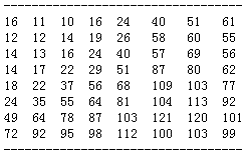
\includegraphics[width=0.3\textwidth]{../Q.png}}
		\subfigure[Canon IXUS 60 (fine)]{
			\label{Fig.sub.2}
			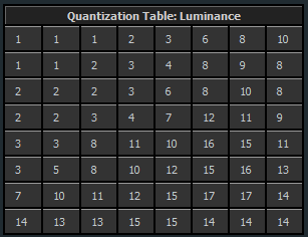
\includegraphics[width=0.3\textwidth]{../Canon.png}}
		\subfigure[Nikon CoolPix L12 (fine)]{
			\label{Fig.sub.3}
			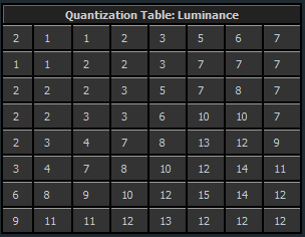
\includegraphics[width=0.3\textwidth]{../Nikon.png}}
		\caption{Different Q(u, v)}
		\label{Fig.Q}
	\end{figure}
	
	
	\subsection{Results}
	
	\subsubsection{With and Without Quantization} 
	先用Jpeg Standard对比使用和不使用Quantization的结果,见\hyperref[Fig.part2-0]{Figure 8}
	
	\begin{figure}[htbp]
		\centering
		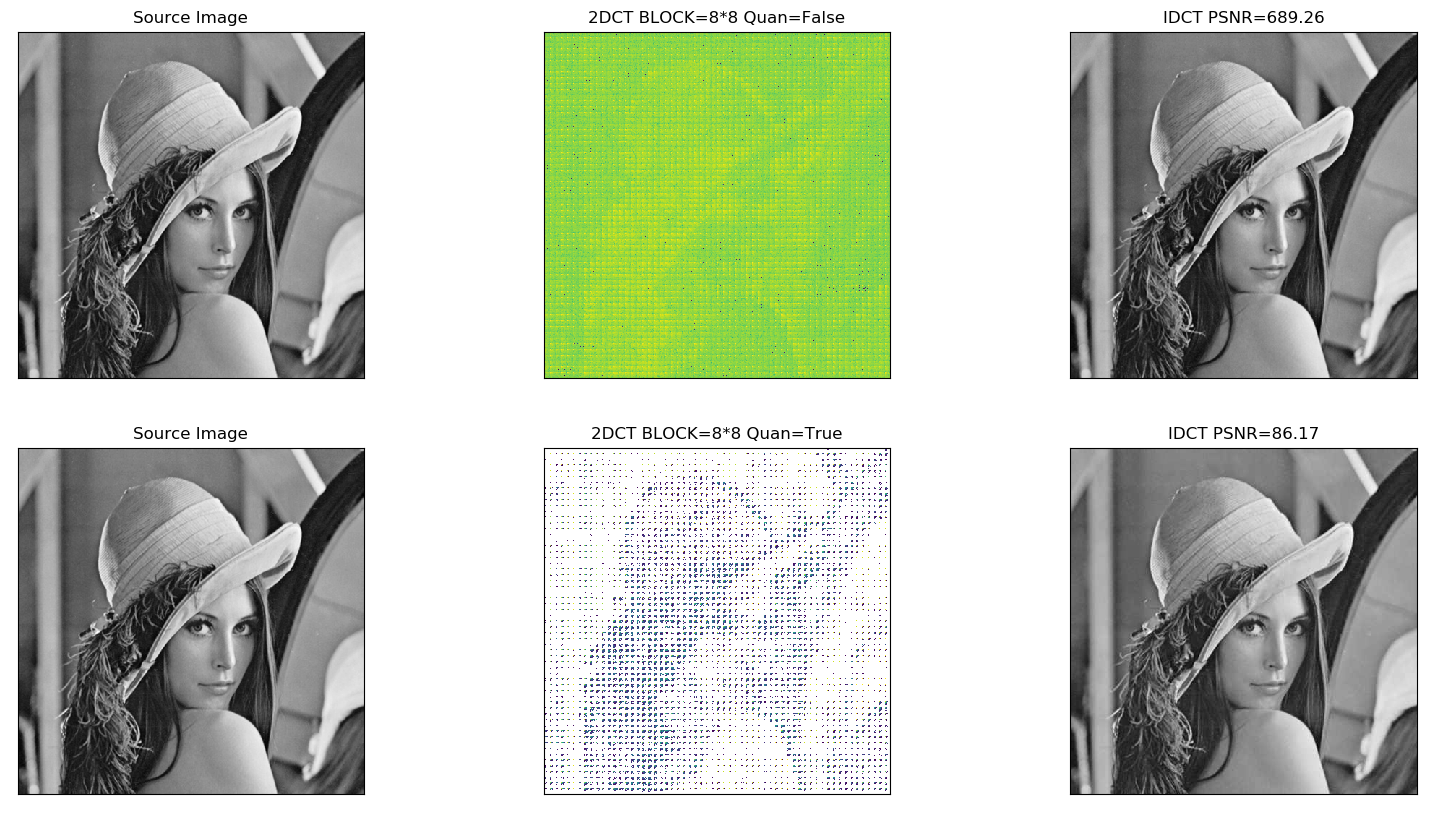
\includegraphics[width=1.0\textwidth]{../part2-0.png}
		\caption{With and Without Quantization}
		\label{Fig.part2-0}
	\end{figure}

	可见Quantization后,DCT明显稀疏了很多,PSNR也下降了不少,这是符合逻辑的。
	
	\subsubsection{Different A and Q} 
	insights部分的不同a*Q(0.1<a<2)和不同Q矩阵的两个任务我整合在了一起见\hyperref[Fig.part2-1]{Figure 9},其中a取值时步幅为0.1
	
	此外对于每种Q,我单独把a等于0.5,1.0和1.5的结果展示出来见\hyperref[Fig.part2-1-0]{Figure 10},以便获得更直观的感受。图片的组织方式是各行之间区别在于使用的Q,从上到下依次是Standard Jpeg,Canon和Nikon,每一行内则包括三组a分别等于0.5,1.0和1.5的DCT和IDCT结果
	
	\begin{figure}[htbp]
		\centering
		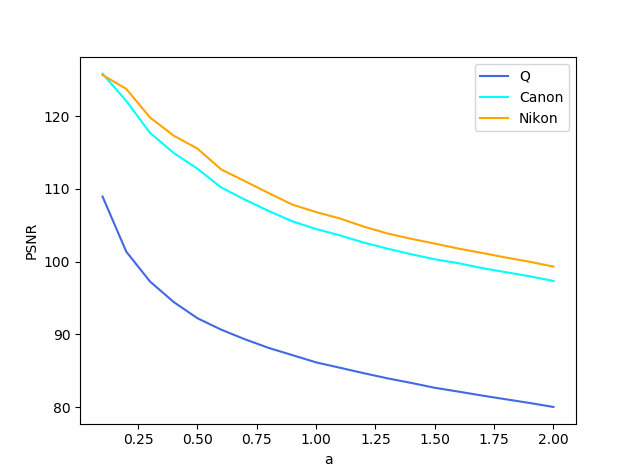
\includegraphics[width=1.0\textwidth]{../part2-1.png}
		\caption{Different A and Q}
		\label{Fig.part2-1}
	\end{figure}
	
	
	\begin{figure}[htbp]
		\centering
		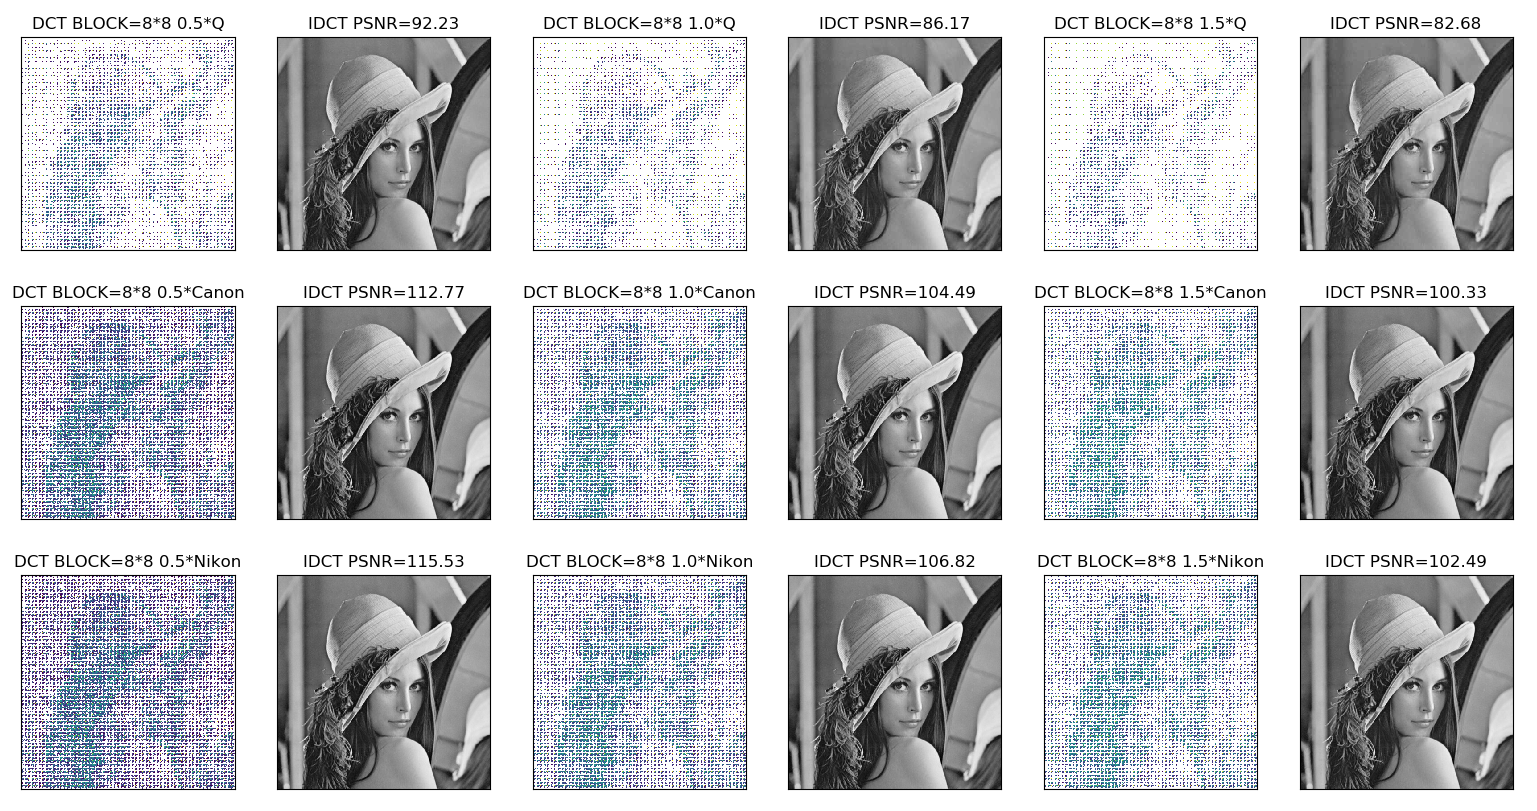
\includegraphics[width=1.0\textwidth]{../part2-1-0.png}
		\caption{Some examples with different A and Q}
		\label{Fig.part2-1-0}
	\end{figure}
	
	\paragraph{A} 单独分析a系数,从折线图可见随着a的增加PSNR是会下降的,从抽取的样例上直观来看,随着a的增加(同一行内从左到右),DCT变得更加稀疏,IDCT的结果观感上变得更加模糊
	
	\paragraph{Q} 单独分析使用的Q矩阵,从折线图可知PSNR值最大的是Nikon,Canon与Nikon相差不大,而Standard Jpeg则和前面两种差得比较远。从抽取的样例直观上来看(同一列从上到下),可见Nikon和Canon的DCT图明显更稀疏,仔细观察IDCT的结果会比Standard Jpeg的IDCT结果更清晰。
	
	我推测Nikon,Canon这两个相机用的Q矩阵相比Standard Jpeg的Q矩阵,会更加注重图片的质量,也即保留更多的DCT信息,以求更高的PSNR,而Standard Jpeg则更侧重图片的压缩这一本职功能,所以会保留更少的DCT信息,以求更高的压缩率。
	
	\section{Conclusion}
	
	总的来说这次小作业和前面三次小作业相比最大的区别在于将图像的处理从时域转到了频域,对我个人来说是很开阔视野的。
	
\end{document}